\documentclass{SelimArticle}
%!TEX root = main.tex

%%%%%%%%%%%%%%%%%%%%%%%%%%%%%%%
% Additional Packages/Options %
%%%%%%%%%%%%%%%%%%%%%%%%%%%%%%%
% \setlist{nosep}
\hypersetup{hidelinks}

%%%%%%%%%%%%%%%%%
% Title Options %
%%%%%%%%%%%%%%%%%
\usepackage{mypage}
\school{McGill University}
\course{Computational Aerodynamics}
\coursenum{MECH 539}
%Add \\[0.3cm] for new line.
\title{Project 5}
\student{Selim \textsc{Belhaouane}}
\studentnum{260450544}
\date{\today}

%%%%%%%%%%%%%%%%%%%%%%%%%
% Additional Formatting %
%%%%%%%%%%%%%%%%%%%%%%%%%
%Horizontal line below section.
\sectionfont{\sectionrule{0pt}{0pt}{-5pt}{0.8pt}}
%Section numbering depth. Value of 2 means numbering ends with subsections.
\setcounter{secnumdepth}{3}
%Table of contents section depth. Same as above.
\setcounter{tocdepth}{2}
\numberwithin{equation}{section}
\numberwithin{figure}{section}

\newcommand{\ra}[1]{\renewcommand{\arraystretch}{#1}}
\newcommand{\pdiff}[2]{\ensuremath{
    \frac{\partial #1}{\partial #2}
}}
\newcommand{\ip}{\ensuremath{_{i+1,j}}}
\newcommand{\im}{\ensuremath{_{i-1,j}}}
\newcommand{\jp}{\ensuremath{_{i,j+1}}}
\newcommand{\jm}{\ensuremath{_{i,j-1}}}
\begin{document}
\mytitlepage
% \tableofcontents
\newpage
% Begin writing here.
\section{Nomenclature}
$N$ is the number of grid points in one direction, i.e. a 400x400 grid corresponds to
$N = 400$.
\section{Governing Differential Equation}
The Laplace equation in two dimensions is given by:
\begin{equation}
    \label{eq:laplace}
    \frac{\partial^2 u}{\partial x^2} + \frac{\partial^2 u}{\partial y^2} = 0
\end{equation}
The boundary conditions are:
\begin{gather*}
    u(x,0) = u(0,y) = u(1,y) = 0\\
    u(x,1) = 1
\end{gather*}

\section{Question 1}
\begin{quote}
    \textit{
     Derive the truncation error for the second-order finite-difference spatial discretization
     for the Laplace equation.}
\end{quote}
A second-order finite-difference spatial discretization for a second derivative is given by:
\begin{equation}
    \label{eq:secord}
    \pdiff{^2u}{x^2} = \frac{u\ip^n - 2 u_{ij}^n + u\im^n}{\Delta x^2}
\end{equation}
Thus, plugging~\Cref{eq:secord} into~\Cref{eq:laplace} yields the following discretization:
\begin{equation}
    \label{eq:laplacediscrete}
    \frac{u\ip^n - 2 u_{ij}^n + u\im^n}{\Delta x^2}
    + \frac{u\jp^n - 2 u_{ij}^n + u\jm^n}{\Delta y^2} = 0
\end{equation}
Now, we substitute each term by its Taylor series expansion into~\Cref{eq:laplacediscrete} to obtain
the modified equation:
\begin{equation*}
    \label{eq:te}
    u_{xx} + u_{yy} =
    \underbrace{
        - \frac{1}{12}\left(u_{xxxx}\Delta x ^2 + u_{yyyy}\Delta y^2 \right)
        + O(\Delta x^4, \Delta y^4)
    }_{\text{Truncation Error}}
\end{equation*}
Note the leading error terms are a function of $\Delta x^2, \Delta y^2$, hence the scheme being
second-order accurate.
\section{Question 2}
\begin{quote}
    \textit{Derive the modified equation for the scheme and note whether the error is dissipative,
    dispersize, or a combination of the two. Explain why?}
\end{quote}
As derived in the previous question, the truncation error is given by:
$$
    \frac{1}{12}\left(u_{xxxx}\Delta x ^2 + u_{yyyy}\Delta y^2 \right)
    + O(\Delta x^4, \Delta y^4)
$$
Due to the discretization, all the odd-order derivatives vanish, leaving only the even-order ones.
Now, we know that a second-order derivative in the truncation error introduces dissipation.
The same can be said of all even-order derivatives.

Thus, the chosen scheme induces dissipative errors \textbf{only}.

\section{Solver Parameters}
Before moving on to the numerical questions, it is important to state all solver parameters.
\begin{description}[noitemsep]
    \item[Programming Language:] Fortran90
    \item[Optimization Level:] O3 (fastest), unless otherwise specified
    \item[Precision:] Single
    \item[Convergence Criteria:] $r^{(k+1)} < 10^{-6}$
    \item[Relaxation Parameter:] 1.5, unless otherwise specified
\end{description}

The residual for each iteration is calculated as:
$$
r^{(k+1)} = \max_{ij}\left( u^{(k+1)}_{ij} - u^{(k)}_{ij} \right)
$$
\section{Question 3}
\begin{quote}
    \textit{Demonstrate the solution of the Laplace Equation for the 400}x\textit{400.}
\end{quote}
The solution of the Laplace Equation is given in~\Cref{fig:q3}.
\begin{figure}[H]
    \centering
    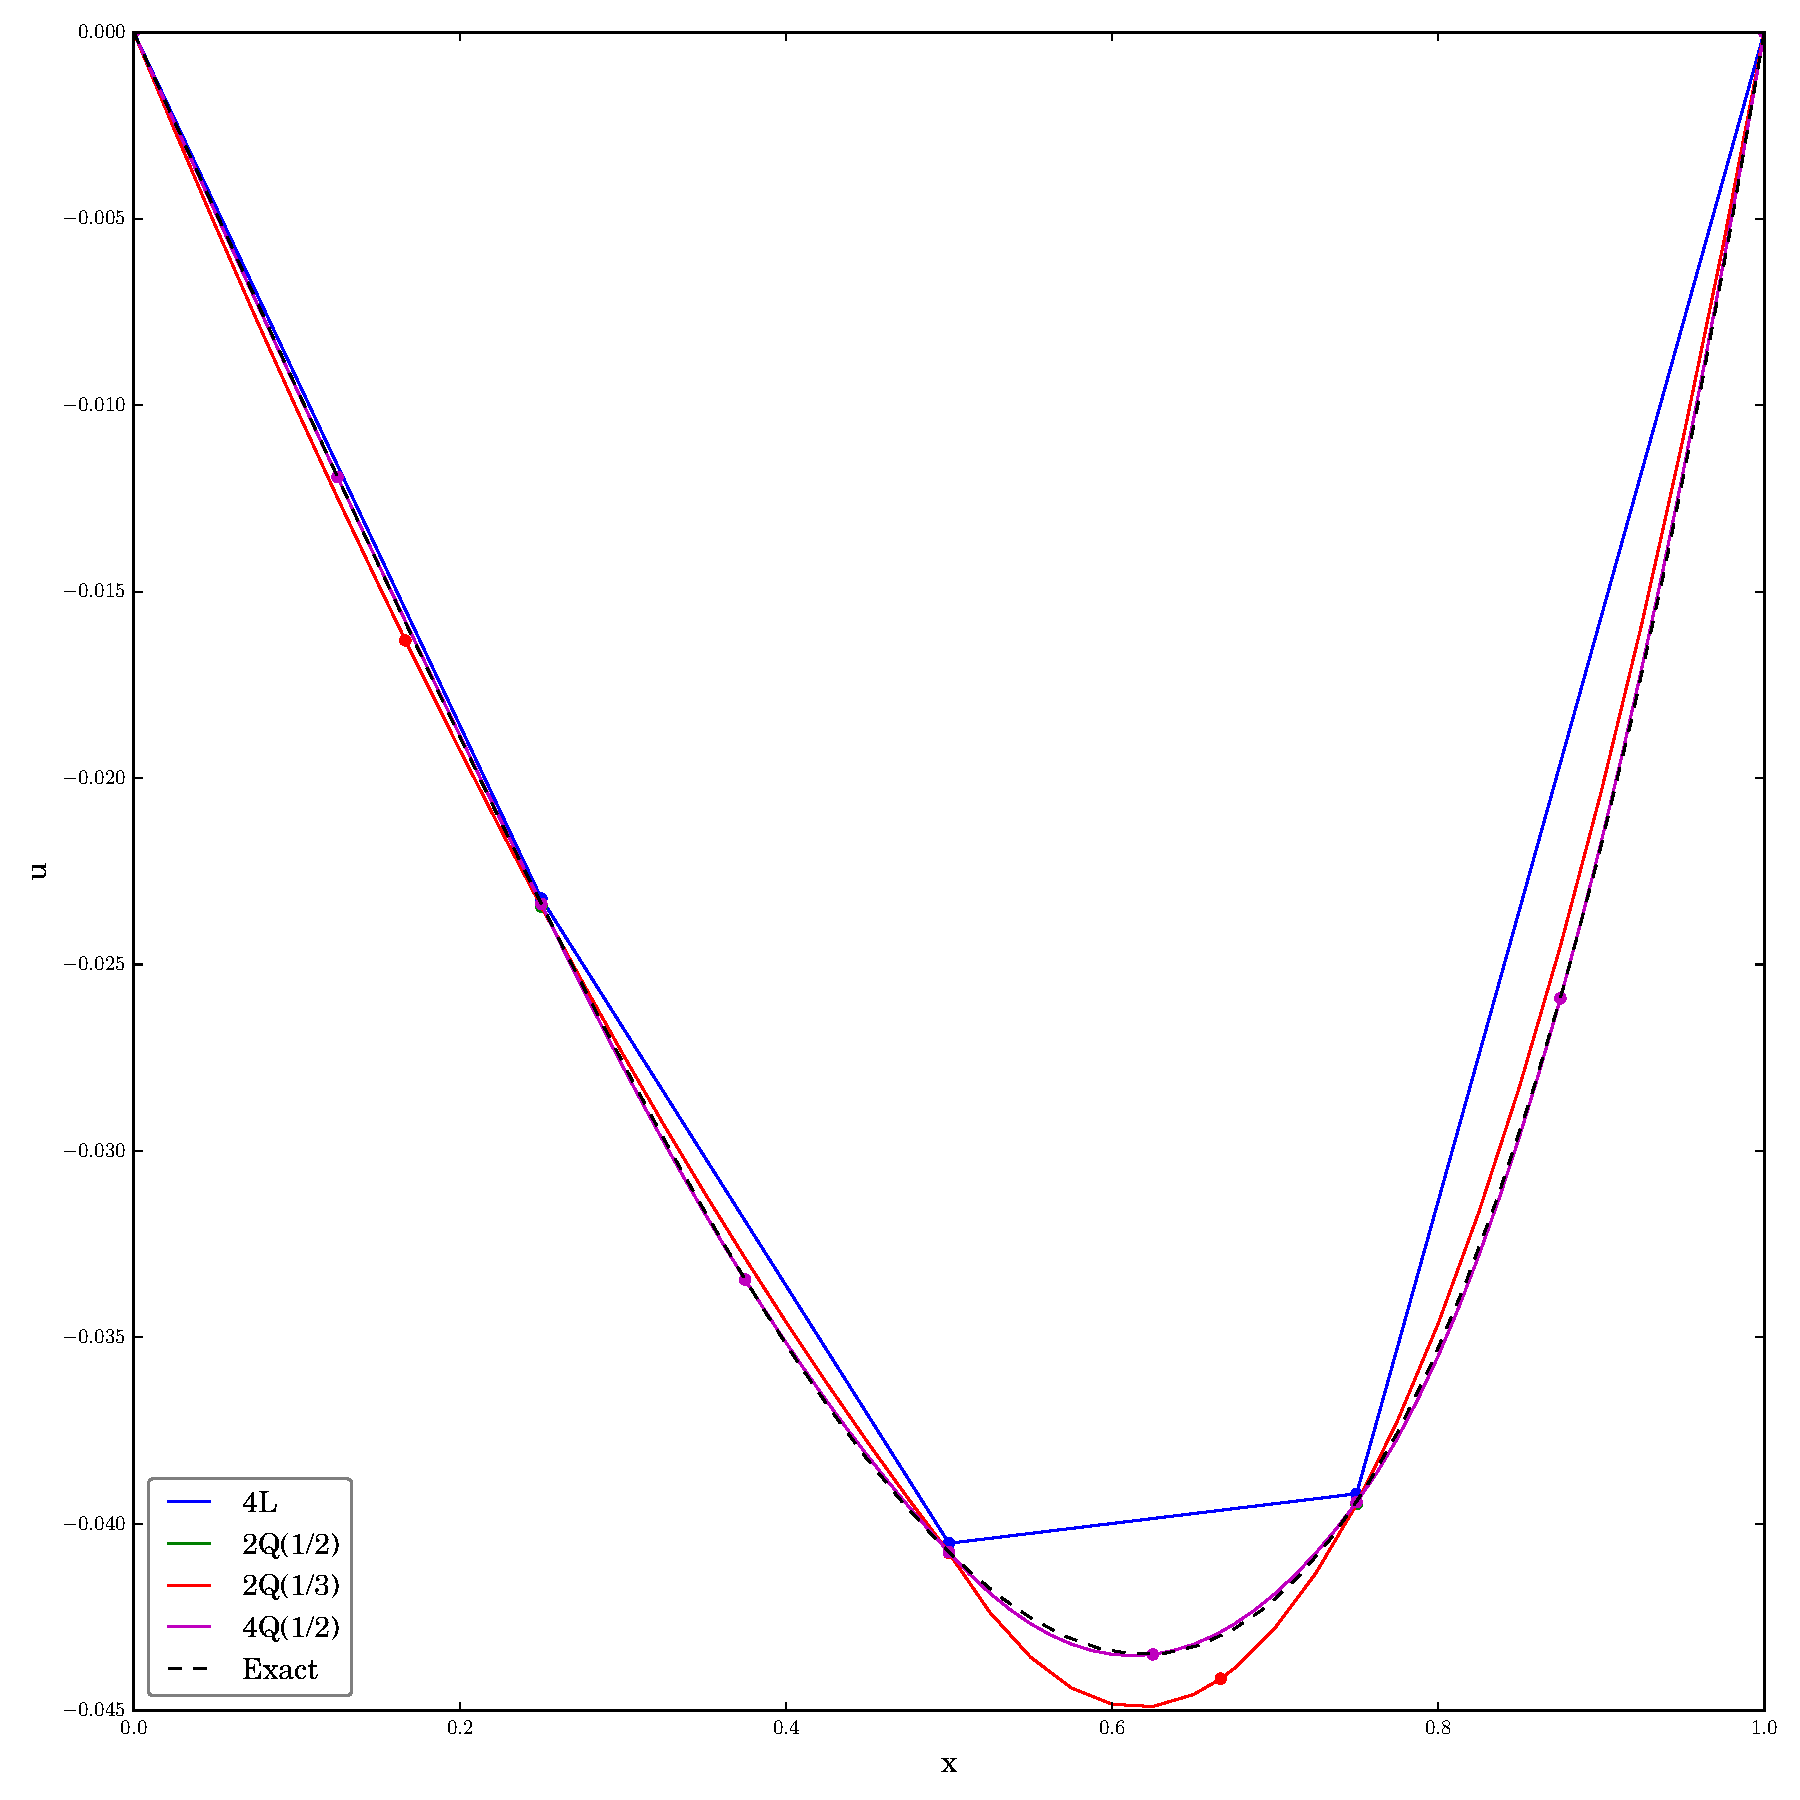
\includegraphics[width=0.8\textwidth]{./figs/q3.pdf}
    \caption{Solution of the Laplace Equation}\label{fig:q3}
\end{figure}

\section{Question 4}
\begin{quote}
\textit{
    Convergence of the residual versus the number of iterations for all three
    methods on the same plot. Provide a plot for each grid size. Discuss the
    difference between the schemes.  Compute the condition number of the
    matrix using the Forsythe-Moler method and discuss the results.
}
\end{quote}
Refer to~\Cref{fig:q4} for the convergence plots.

\subsection{Effect of scheme on convergence}
It can be seen that the Jacobi scheme is consistently slower to converge than the other schemes, whereas
SOR is the fastest. However the chosen relaxation parameter plays a significant role in the convergence rate
for the latter scheme, as will be shown for Question 7.

It is not a surprise that the Gauss-Siedel scheme is faster than Jacobi due to the former using
more up-to-date information, i.e. $u^{(k+1)}$ values.

Again, the reason for SOR's even faster convergence rate is given in Question 7.

\subsection{Effect of grid size on convergence}
From a purely physical point of view, one would expect the number of iterations required to converge
to increase with the number of grid points since information takes longer to travel the grid. Specifically,
in the case of the Jacobi method, the correction for $u_{ij}$ is only a function of the five neighboring
nodes.

\subsection{Condition number}

Of course, the number of iterations required to converge increases with the number of grid points, since it takes longer for information
to travel the grid.
\begin{figure}
    \centering
    \includegraphics[width=1.0\textwidth]{./figs/q4.pdf}
    \caption{Convergence history comparison between methods for grid sizes: 100x100, 200x200, 400x400 -- going from top to bottom.}\label{fig:q4}
\end{figure}

\section{Question 5}
\begin{quote}
    \textit{Convergence of the residual versus the CPU time for all three methods on the same
        plot. Discuss the difference between the schemes. Comment on the number of vectors
        and arrays that were necessary for each scheme and compare the algorithms in terms
        of memory usage.}
\end{quote}
The convergence of the residual versus CPU time of all three methods for the 400x400 grid is shown
in~\Cref{fig:resvscpu}.

\subsection{Effect of scheme on CPU time}
One immediately notices Jacobi's consistenly faster convergence in terms of CPU time. Indeed, this is
quite peculiar. This is not the expected behavior for the following reasons:
\begin{itemize}[noitemsep]
    \item The Gauss scheme converges approximately at twice the rate of Jacobi in terms of iterations. In other hands,
        Jacobi requires double the number of iterations to converge.
    \item The Gauss scheme requires storage of only one array for $u$. I doubt this would, however, significantly
        impact performance in this case since both $u$ arrays can easily fit in L3 cache
        (see Appendix for a brief discussion of this).
\end{itemize}
For completeness, and to remove doubt in the reader's mind that the program structure
is to blame, the relevant part of the code is included in Listing~\ref{lst:fortran}, found in the Appendix.

\subsubsection{Fortran optimization}
So what could the explanation be? Well, there's a good reason why the Fortran optimizing compiler
is amongst the top ten algorithms of the 20th century. \Cref{tab:performance} illustrates the
effects of optimization level on performance for the Jacobi and Gauss schemes. There are four
optimization levels available to the compiled (gfortran) used. In order of ascending
optimization, these are: g, O1, O2 and O3. Finally, $N$ is taken to be the size of the grid, i.e.
the number of grid points in the $x$ and $y$ direction.
\newcommand{\mct}[1]{\multicolumn{2}{c}{#1}}
\newcommand{\pht}{\phantom{a}}
\newcommand{\mrt}[1]{\multirow{4}{*}{#1}}
\begin{table}[H]
\caption{Performance comparison of Gauss and Jacobi using different
optimization levels. All runs converged with a tolerance of
$10^{-6}$.}
\label{tab:performance}
\centering
\begin{tabular}{@{}r cc c cc c cc @{}}
    \toprule
    & \mct{Iterations} & \pht & \mct{Time per Iteration} & \pht & \mct{Total Time}\\
    &         &        & \pht & \mct{($10^{-5}$ s)}        & \pht & \mct{(s)}       \\
    \cmidrule{2-3} \cmidrule{5-6} \cmidrule {8-9}
     & Jacobi & Gauss && Jacobi & Gauss && Jacobi & Gauss\\
    \midrule

$N = 100$\\
     g & \mrt{10726} & \mrt{6020} && 24 & 23 &&  2.53 &  1.38 \\
    O1 &  &  && 8 & 9 &&  0.91 &  0.53 \\
    O2 &  &  && 6 & 7 &&  0.68 &  0.41 \\
    O3 &  &  && 4 & 6 &&  0.38 &  0.39 \\
$N = 200$\\
     g & \mrt{31851} & \mrt{18684} && 93 & 93 &&  29.7 &  17.3 \\
    O1 &  &  && 34 & 35 &&  10.7 &   6.6 \\
    O2 &  &  && 25 & 27 &&   8.1 &   5.1 \\
    O3 &  &  && 14 & 26 &&   4.5 &   4.9 \\
$N = 400$\\
     g & \mrt{83206} & \mrt{52634} && 375 & 371 &&   312 &   195 \\
    O1 &  &  && 135 & 142 &&   112 &    75 \\
    O2 &  &  && 102 & 109 &&    85 &    58 \\
    O3 &  &  && 57 & 107 &&    47 &    56 \\

    \bottomrule
\end{tabular}
\end{table}

Something incredible happens when the optimization is switched from O2 to O3: the time
per iteration for Jacobi, and only Jacobi, drops down significantly. This performance increase is
enough to bring Jacobi's total time below that of Gauss, despite the discrepancy in number of
iterations.

While the exact reason for this behavior is way beyond the scope of this course, I dare hypothesize
that the Fortran compiler figures out that \texttt{uold} is not modified after the initial
assignment at line 11, which allows for efficient \textit{prefetching}.

Now, if the code were written in MATLAB or Python, I certainly wouldn't expect this to be possible.
Consequently, were it not for the optimization, the total CPU time should merely be a function of
the number of iterations and the time per iteration should be roughly the same for Jacobi and Gauss,
as is the case for optimization level $g$.

\subsubsection{Parallelization}
It's worth noting that only the Jacobi scheme can be parallelized, which would further decrease
the time per iteration for large enough grids.

\subsection{Memory usage}
As mentioned above, Gauss and SOR require only one $u$ vector to be stored, which is of length $N^2$. On
the other hand, Jacobi requires two of those $u$ vectors to be stored. In fact, looking at the memory usage
for the process shows exactly that.

\section{Question 7}
In all previous questions, SOR essentially acted as an over-relaxed Gauss scheme. This leads to quicker
convergence, since the "correction" at each point is attributed a greater weight.
In other words, values are allowed to vary faster. Of course, over-relaxation is not the
best choice for every problem. In fact, under-relaxation is often necessary when dealing with stiff
problems. A more detailed discussion on relaxation is, however, beyond the scope of this assignment and course.

\newpage
\appendix
\section{Appendix}
\subsection{Linear Solver Code}

\lstset{language=[90]Fortran,
  basicstyle=\footnotesize\ttfamily,
  lineskip=-2pt,
  frame=single,
  keywordstyle=\color{blue},
  commentstyle=\color{PineGreen},
  numbers=left,
  morecomment=[l]{!\ }% Comment only with space after !
}
The listing below shows the meat of the code.
\texttt{implicit none} is used,
which means all undeclared variables that appear in the listing are globals.
These globals are all constants.
\begin{lstlisting}[caption={Relevant part of the linear solver.
\texttt{solverID} is a global integer variable that has the mapping:
1=Jacobi, 2=Gauss, 3=SOR},
label=lst:fortran]
subroutine update(u, maxerr)
    real(sp), dimension(:), intent(inout) :: u
    real(sp), intent(out) :: maxerr
    real(sp), allocatable, dimension(:) :: uold
    real(sp) :: s, corr, err
    integer, dimension(4) :: stencil
    integer :: i, j, row
    maxerr = 0
    if (solverID .eq. 1) then
        allocate(uold(size(u)))
        uold = u
    end if
    do i = 1, nx
        do j = 1, nx
            if (is_bc(i,j)) then
                cycle
            end if
            row = get_row(i, j)
            ! Calculate correction
            stencil = (/ row-nx, row-1, row+1, row+nx /)
            if (solverID .eq. 1) then
                s = sum(uold(stencil))
            else
                s = sum(u(stencil))
            end if
            corr = (BI - AIJ*s)/AII
            if (solverID .eq. 3) then
                corr = (1.0 - relax)*u(row) + relax*corr
            end if
            ! Calculate error
            err = abs(corr - u(row))
            maxerr = max(maxerr, err)
            ! Assign correction
            u(row) = corr
        end do
    end do
end subroutine
\end{lstlisting}

\subsection{Cache Calculations}
These are rough calculations and based on my limited computer science knowledge.

My personal computer has an L3 cache size of 6MB. For a $N = 400$ problem, a $u$ array is of length $400^2$.
Using single precision -- a single precision floating point number takes up 4 bytes -- this means $u$ takes up
0.64MB.  Thus, storing an additional \texttt{uold} array should not be a problem.

I also tried bumping $N$ up to 1000 -- which brings the size of $u$ to 4MB -- and Jacobi
was \textit{still} faster than Gauss at O3, although the time per iteration ratio (Gauss/Jacobi) increased
from 0.53 (for $N = 400$) to 0.73, meaning the optimization was not as significant. However, Jacobi wasn't any
slower than Gauss at O2 or O1 either.

Thus, all we can conclude is that my understanding of cache is not great and that increasing $N$ will
apparently not make Jacobi slower.
\end{document}
